\documentclass{article}
\usepackage[utf8]{inputenc}
\usepackage{geometry}
\usepackage{longtable}
\usepackage{xcolor}
\usepackage{booktabs}
\usepackage{listings}
\usepackage{pdfpages} % Added for including external PDFs
\geometry{a4paper, margin=1in}

\lstset{
    basicstyle=\ttfamily\scriptsize,
    breaklines=true,
    breakatwhitespace=false,
    frame=single,
    showstringspaces=false
}

\title{MEA API Test Report}
\author{Automated Test Suite}
\date{\today}

\begin{document}

\maketitle

\section{Summary}
\begin{itemize}
    \item \textbf{Total Tests:} 9
    \item \textbf{Passed:} 9
    \item \textbf{Failed:} 0
    \item \textbf{Errors:} 0
    \item \textbf{Skipped:} 0
    \item \textbf{Total Duration:} 5.116 seconds
\end{itemize}

\section{Detailed Results}
\begin{longtable}{p{0.6\textwidth} p{0.2\textwidth} p{0.1\textwidth}}
\toprule
\textbf{Test Case} & \textbf{Status} & \textbf{Time (s)} \\
\midrule
\endhead
test\_00\_connection\_setup & \textcolor{green}{Pass} & 2.005 \\
test\_remote\_start\_transaction & \textcolor{green}{Pass} & 0.441 \\
test\_remote\_stop\_transaction & \textcolor{green}{Pass} & 0.463 \\
test\_reserve\_now & \textcolor{green}{Pass} & 0.361 \\
test\_cancel\_reservation & \textcolor{green}{Pass} & 0.341 \\
test\_change\_configuration & \textcolor{green}{Pass} & 0.340 \\
test\_set\_charging\_profile & \textcolor{green}{Pass} & 0.363 \\
test\_remote\_reset & \textcolor{green}{Pass} & 0.358 \\
test\_get\_configuration & \textcolor{green}{Pass} & 0.346 \\
\bottomrule
\end{longtable}

\section{Global Execution Log}
\begin{lstlisting}
============================= test session starts ==============================
platform darwin -- Python 3.12.3, pytest-9.0.2, pluggy-1.6.0 -- /Library/Frameworks/Python.framework/Versions/3.12/bin/python3
cachedir: .pytest_cache
rootdir: /Users/rus/development/MEA-V2G
collecting ... collected 9 items

tests/api/test_mea_postman.py::test_00_connection_setup DEBUG: conftest PACKET_QUEUE ID: 4521171264

[EVSE] RAW RECV: [3,"51da25ab-c8f9-42f8-b010-7489f20fa2b1",{"currentTime":"2026-01-10T01:41:10Z","interval":3600,"status":"Accepted"}]

[EVSE] BootNotification ACCEPTED

[EVSE] RAW RECV: [3,"33122203-af6b-4e35-ab9a-573179bcac00",{}]

[EVSE] StatusNotification ACKNOWLEDGED (Available)

[EVSE] RAW RECV: [3,"bb97059e-d083-461a-9fab-82bb55cdf1ea",{}]

[EVSE] StatusNotification ACKNOWLEDGED (Available)

[EVSE] RAW RECV: [3,"5e561267-d566-4271-9128-a9842eae540e",{"idTagInfo":{"expiryDate":"2031-01-30T12:00:44Z","parentIdTag":"pid2025","status":"Accepted"}}]

[EVSE] Authorize ACKNOWLEDGED (Accepted)

[EVSE] RAW RECV: [3,"f7d40a9d-2b43-4e89-b0cb-91d66a3d9ea0",{}]

[EVSE] StatusNotification ACKNOWLEDGED (Preparing)

[EVSE] RAW RECV: [3,"b0afe81b-f478-40b3-ba20-65f84527cf26",{"currentTime":"2026-01-10T01:41:11Z"}]

[EVSE] Heartbeat ACKNOWLEDGED (Time: 2026-01-10T01:41:11Z)

--- TEST CASE: Connection Setup ---
Waiting for EVSE to initialize...
--- EVSE Interactions ---
[EVSE] Connected to CSMS!
[EVSE] Sending BootNotification...
[EVSE] RAW RECV: [3,"51da25ab-c8f9-42f8-b010-7489f20fa2b1",{"currentTime":"2026-01-10T01:41:10Z","interval":3600,"status":"Accepted"}]
[EVSE] BootNotification ACCEPTED
[EVSE] Sending StatusNotification (Available)...
[EVSE] RAW RECV: [3,"33122203-af6b-4e35-ab9a-573179bcac00",{}]
[EVSE] StatusNotification ACKNOWLEDGED (Available)
[EVSE] Sending StatusNotification (Connector 1: Available)...
[EVSE] RAW RECV: [3,"bb97059e-d083-461a-9fab-82bb55cdf1ea",{}]
[EVSE] StatusNotification ACKNOWLEDGED (Available)
[EVSE] Sending Authorize (RFID_SIM)...
[EVSE] RAW RECV: [3,"5e561267-d566-4271-9128-a9842eae540e",{"idTagInfo":{"expiryDate":"2031-01-30T12:00:44Z","parentIdTag":"pid2025","status":"Accepted"}}]
[EVSE] Authorize ACKNOWLEDGED (Accepted)
[EVSE] Sending StatusNotification (Connector 1: Preparing)...
[EVSE] RAW RECV: [3,"f7d40a9d-2b43-4e89-b0cb-91d66a3d9ea0",{}]
[EVSE] StatusNotification ACKNOWLEDGED (Preparing)
[EVSE] Sending Heartbeat...
[EVSE] RAW RECV: [3,"b0afe81b-f478-40b3-ba20-65f84527cf26",{"currentTime":"2026-01-10T01:41:11Z"}]
[EVSE] Heartbeat ACKNOWLEDGED (Time: 2026-01-10T01:41:11Z)
--------------------------------
SUCCESS: BootNotification was accepted.
PASSED
tests/api/test_mea_postman.py::test_remote_start_transaction 
[EVSE] RAW RECV: [2,"71a00c1bedc511f089330242c0a8300e","RemoteStartTransaction",{"connectorId":1,"idTag":"RFID_SIM"}]

[EVSE] RECV Packet: RemoteStartTransaction
Payload: {
  "idTag": "RFID_SIM",
  "connectorId": 1
}

[EVSE] Sending RemoteStartTransaction Response (Accepted)

[EVSE] RAW RECV: [3,"deefd530-f275-4a77-8f8c-c6a1f16348a9",{"idTagInfo":{"expiryDate":"2031-01-30T12:00:44Z","parentIdTag":"pid2025","status":"Accepted"},"transactionId":7359}]

--- TEST CASE: Remote Start Transaction ---
API Request: POST https://ocppapi.measandbox.com/EV/cmd/chargepoint/remoteStart
Payload: {
  "chargepoint_id": "rddQC4000001",
  "connector_id": 1,
  "card_id": "RFID_SIM"
}
Response Code: 200
Response Body: {
  "status": "OK",
  "code": 200,
  "messages": "OK",
  "server-time": "2026-01-10T01:41:11Z",
  "result": {
    "status": true,
    "transaction_id": "7359"
  }
}
--- EVSE Interactions ---
[EVSE] RAW RECV: [2,"71a00c1bedc511f089330242c0a8300e","RemoteStartTransaction",{"connectorId":1,"idTag":"RFID_SIM"}]
--------------------------------
CAPTURED TRANSACTION ID: 7359
PASSED
tests/api/test_mea_postman.py::test_remote_stop_transaction Loaded Transaction ID from file: 7359

[EVSE] RAW RECV: [2,"71e5623eedc511f085320242c0a8300e","RemoteStopTransaction",{"transactionId":7359}]

[EVSE] RECV Packet: RemoteStopTransaction
Payload: {
  "transactionId": 7359
}

[EVSE] Sending RemoteStopTransaction Response (Accepted)

[EVSE] RAW RECV: [3,"f78c27e0-d4ae-4040-b313-5860beaa1832",{}]

[EVSE] StatusNotification ACKNOWLEDGED (Finishing)

[EVSE] RAW RECV: [3,"62a0e40e-e41d-46aa-b788-9032f66750be",{}]

[EVSE] RAW RECV: [3,"dad79cbc-e30b-411d-a1d2-c9c381d051a9",{}]

[EVSE] StatusNotification ACKNOWLEDGED (Available)

--- TEST CASE: Remote Stop Transaction ---
API Request: POST https://ocppapi.measandbox.com/EV/cmd/chargepoint/remoteStop
Payload: {
  "chargepoint_id": "rddQC4000001",
  "transaction_id": 7359
}
Response Code: 200
Response Body: {
  "status": "OK",
  "code": 200,
  "messages": "OK",
  "server-time": "2026-01-10T01:41:12Z",
  "result": {
    "transaction_id": 7359,
    "start_time": "2026-01-10T01:40:03Z",
    "stop_time": "2026-01-10T01:40:03Z",
    "kWh": 0.1
  }
}
--- EVSE Interactions ---
[EVSE] RECV Packet: RemoteStartTransaction
Payload: {
  "idTag": "RFID_SIM",
  "connectorId": 1
}
[EVSE] Sending RemoteStartTransaction Response (Accepted)
[EVSE] RAW RECV: [3,"deefd530-f275-4a77-8f8c-c6a1f16348a9",{"idTagInfo":{"expiryDate":"2031-01-30T12:00:44Z","parentIdTag":"pid2025","status":"Accepted"},"transactionId":7359}]
[EVSE] RAW RECV: [2,"71e5623eedc511f085320242c0a8300e","RemoteStopTransaction",{"transactionId":7359}]
--------------------------------
PASSED
tests/api/test_mea_postman.py::test_reserve_now 
[EVSE] RAW RECV: [2,"722fe40cedc511f0910f0242c0a8300e","ReserveNow",{"connectorId":1,"expiryDate":"2026-01-10T01:56:12Z","idTag":"RFID_SIM","parentIdTag":"pid2025","reservationId":981}]

[EVSE] RECV Packet: ReserveNow
Payload: {
  "reservationId": 981,
  "expiryDate": "2026-01-10T01:56:12Z",
  "idTag": "RFID_SIM",
  "connectorId": 1,
  "parent_id_tag": "pid2025"
}

[EVSE] Sending ReserveNow Response (Accepted)

--- TEST CASE: Reserve Now ---
API Request: POST https://ocppapi.measandbox.com/EV/cmd/chargepoint/reserve
Payload: {
  "chargepoint": "rddQC4000001",
  "connector": 1,
  "duration": 15,
  "card_id": "RFID_SIM"
}
Response Code: 200
Response Body: {
  "status": "OK",
  "code": 200,
  "messages": "OK",
  "server-time": "2026-01-10T01:41:12Z",
  "result": {
    "status": "Accepted",
    "reservation_id": 981
  }
}
--- EVSE Interactions ---
[EVSE] RECV Packet: RemoteStopTransaction
Payload: {
  "transactionId": 7359
}
[EVSE] Sending RemoteStopTransaction Response (Accepted)
[EVSE] RAW RECV: [3,"f78c27e0-d4ae-4040-b313-5860beaa1832",{}]
[EVSE] StatusNotification ACKNOWLEDGED (Finishing)
[EVSE] RAW RECV: [3,"62a0e40e-e41d-46aa-b788-9032f66750be",{}]
[EVSE] RAW RECV: [3,"dad79cbc-e30b-411d-a1d2-c9c381d051a9",{}]
[EVSE] StatusNotification ACKNOWLEDGED (Available)
[EVSE] RAW RECV: [2,"722fe40cedc511f0910f0242c0a8300e","ReserveNow",{"connectorId":1,"expiryDate":"2026-01-10T01:56:12Z","idTag":"RFID_SIM","parentIdTag":"pid2025","reservationId":981}]
--------------------------------
CAPTURED RESERVATION ID: 981
PASSED
tests/api/test_mea_postman.py::test_cancel_reservation Loaded Reservation ID from file: 981

[EVSE] RAW RECV: [2,"7260abceedc511f098000242c0a8300e","CancelReservation",{"reservationId":981}]

[EVSE] RECV Packet: CancelReservation
Payload: {
  "reservationId": 981
}

[EVSE] Sending CancelReservation Response (Accepted)

--- TEST CASE: Cancel Reservation ---
API Request: POST https://ocppapi.measandbox.com/EV/cmd/chargepoint/cancel
Payload: {
  "chargepoint": "rddQC4000001",
  "reservation_id": 981
}
Response Code: 200
Response Body: {
  "status": "OK",
  "code": 200,
  "messages": "OK",
  "server-time": "2026-01-10T01:41:13Z",
  "result": {
    "status": "Accepted",
    "reservation_id": 981
  }
}
--- EVSE Interactions ---
[EVSE] RECV Packet: ReserveNow
Payload: {
  "reservationId": 981,
  "expiryDate": "2026-01-10T01:56:12Z",
  "idTag": "RFID_SIM",
  "connectorId": 1,
  "parent_id_tag": "pid2025"
}
[EVSE] Sending ReserveNow Response (Accepted)
[EVSE] RAW RECV: [2,"7260abceedc511f098000242c0a8300e","CancelReservation",{"reservationId":981}]
--------------------------------
PASSED
tests/api/test_mea_postman.py::test_change_configuration 
[EVSE] RAW RECV: [2,"7293715bedc511f083700242c0a8300e","ChangeConfiguration",{"key":"test","value":"1"}]

[EVSE] RECV Packet: ChangeConfiguration
Payload: {
  "key": "test",
  "value": "1"
}

--- TEST CASE: Change Configuration ---
API Request: POST https://ocppapi.measandbox.com/EV/remote/changeConfiguration
Payload: {
  "chargepoint_id": "rddQC4000001",
  "key": "test",
  "value": "1"
}
Response Code: 200
Response Body: {
  "status": "OK",
  "code": 200,
  "messages": "OK",
  "server-time": "2026-01-10T01:41:13Z",
  "result": {
    "status": "Accepted"
  }
}
--- EVSE Interactions ---
[EVSE] RECV Packet: CancelReservation
Payload: {
  "reservationId": 981
}
[EVSE] Sending CancelReservation Response (Accepted)
[EVSE] RAW RECV: [2,"7293715bedc511f083700242c0a8300e","ChangeConfiguration",{"key":"test","value":"1"}]
--------------------------------
PASSED
tests/api/test_mea_postman.py::test_set_charging_profile 
[EVSE] RAW RECV: [2,"72c9027eedc511f080190242c0a8300e","SetChargingProfile",{"connectorId":1,"csChargingProfiles":{"chargingProfileId":99,"chargingProfileKind":"Absolute","chargingProfilePurpose":"TxProfile","chargingSchedule":{"chargingRateUnit":"A","chargingSchedulePeriod":[{"limit":20,"numberPhases":1,"startPeriod":1}],"duration":6000,"minChargingRate":1,"startSchedule":"2026-01-10T01:45:33.750601Z"},"recurrencyKind":"Daily","stackLevel":1,"transactionId":7337,"validFrom":"2026-01-09T01:40:33.750601Z","validTo":"2027-01-10T01:40:33.750601Z"}}]

[EVSE] RECV Packet: SetChargingProfile
Payload: {
  "connectorId": 1,
  "csChargingProfiles": {
    "charging_profile_id": 99,
    "charging_profile_kind": "Absolute",
    "charging_profile_purpose": "TxProfile",
    "charging_schedule": {
      "charging_rate_unit": "A",
      "charging_schedule_period": [
        {
          "limit": 20,
          "number_phases": 1,
          "start_period": 1
        }
      ],
      "duration": 6000,
      "min_charging_rate": 1,
      "start_schedule": "2026-01-10T01:45:33.750601Z"
    },
    "recurrency_kind": "Daily",
    "stack_level": 1,
    "transaction_id": 7337,
    "valid_from": "2026-01-09T01:40:33.750601Z",
    "valid_to": "2027-01-10T01:40:33.750601Z"
  }
}

[EVSE] Sending SetChargingProfile Response (Accepted)

--- TEST CASE: Set Charging Profile ---
API Request: POST https://ocppapi.measandbox.com/EV/remote/SetChargingProfile
Payload: {
  "chargepoint_id": "rddQC4000001",
  "connectorId": 1,
  "csChargingProfiles": {
    "chargingProfileId": 99,
    "transactionId": 7337,
    "stackLevel": 1,
    "chargingProfilePurpose": "TxProfile",
    "chargingProfileKind": "Absolute",
    "recurrencyKind": "Daily",
    "validFrom": "2026-01-09T01:40:33.750601Z",
    "validTo": "2027-01-10T01:40:33.750601Z",
    "chargingSchedule": {
      "duration": 6000,
      "startSchedule": "2026-01-10T01:45:33.750601Z",
      "chargingRateUnit": "A",
      "minChargingRate": 1,
      "chargingSchedulePeriod": [
        {
          "startPeriod": 1,
          "limit": 20,
          "numberPhases": 1
        }
      ]
    }
  }
}
Response Code: 200
Response Body: {
  "status": "OK",
  "code": 200,
  "messages": "OK",
  "server-time": "2026-01-10T01:41:13Z",
  "result": {
    "status": "Accepted"
  }
}
--- EVSE Interactions ---
[EVSE] RECV Packet: ChangeConfiguration
Payload: {
  "key": "test",
  "value": "1"
}
[EVSE] RAW RECV: [2,"72c9027eedc511f080190242c0a8300e","SetChargingProfile",{"connectorId":1,"csChargingProfiles":{"chargingProfileId":99,"chargingProfileKind":"Absolute","chargingProfilePurpose":"TxProfile","chargingSchedule":{"chargingRateUnit":"A","chargingSchedulePeriod":[{"limit":20,"numberPhases":1,"startPeriod":1}],"duration":6000,"minChargingRate":1,"startSchedule":"2026-01-10T01:45:33.750601Z"},"recurrencyKind":"Daily","stackLevel":1,"transactionId":7337,"validFrom":"2026-01-09T01:40:33.750601Z","validTo":"2027-01-10T01:40:33.750601Z"}}]
--------------------------------
PASSED
tests/api/test_mea_postman.py::test_remote_reset 
[EVSE] RAW RECV: [2,"73028208edc511f09f150242c0a8300e","Reset",{"type":"Soft"}]

[EVSE] RECV Packet: Reset
Payload: {
  "type": "Soft"
}

[EVSE] Sending Reset Response (Accepted)

--- TEST CASE: Remote Reset ---
API Request: POST https://ocppapi.measandbox.com/EV/remote/reset
Payload: {
  "chargepoint": "rddQC4000001",
  "reset_type": "Soft"
}
Response Code: 200
Response Body: {
  "status": "OK",
  "code": 200,
  "messages": "OK",
  "server-time": "2026-01-10T01:41:14Z",
  "result": {
    "status": "Accepted"
  }
}
--- EVSE Interactions ---
[EVSE] RECV Packet: SetChargingProfile
Payload: {
  "connectorId": 1,
  "csChargingProfiles": {
    "charging_profile_id": 99,
    "charging_profile_kind": "Absolute",
    "charging_profile_purpose": "TxProfile",
    "charging_schedule": {
      "charging_rate_unit": "A",
      "charging_schedule_period": [
        {
          "limit": 20,
          "number_phases": 1,
          "start_period": 1
        }
      ],
      "duration": 6000,
      "min_charging_rate": 1,
      "start_schedule": "2026-01-10T01:45:33.750601Z"
    },
    "recurrency_kind": "Daily",
    "stack_level": 1,
    "transaction_id": 7337,
    "valid_from": "2026-01-09T01:40:33.750601Z",
    "valid_to": "2027-01-10T01:40:33.750601Z"
  }
}
[EVSE] Sending SetChargingProfile Response (Accepted)
[EVSE] RAW RECV: [2,"73028208edc511f09f150242c0a8300e","Reset",{"type":"Soft"}]
--------------------------------
PASSED
tests/api/test_mea_postman.py::test_get_configuration 
[EVSE] RAW RECV: [2,"73376101edc511f0951d0242c0a8300e","GetConfiguration",{"key":[]}]

[EVSE] RECV Packet: GetConfiguration
Payload: {
  "keys": null,
  "key": []
}

[EVSE] Sending GetConfiguration Response (Count: 7)

--- TEST CASE: Get Configuration ---
API Request: POST https://ocppapi.measandbox.com/EV/cmd/chargepoint/getConfiguration
Payload: {
  "chargepoint": "rddQC4000001",
  "key": []
}
Response Code: 200
Response Body: {
  "status": "OK",
  "code": 200,
  "messages": "OK",
  "server-time": "2026-01-10T01:41:14Z",
  "result": {
    "configurationKey": [
      {
        "key": "HeartbeatInterval",
        "readonly": false,
        "value": "60"
      },
      {
        "key": "ConnectionTimeOut",
        "readonly": false,
        "value": "60"
      },
      {
        "key": "MeterValueSampleInterval",
        "readonly": false,
        "value": "60"
      },
      {
        "key": "LocalAuthorizeOffline",
        "readonly": false,
        "value": "False"
      },
      {
        "key": "UnlockConnectorOnEVSideDisconnect",
        "readonly": false,
        "value": "False"
      },
      {
        "key": "AutoCharge",
        "readonly": false,
        "value": "False"
      },
      {
        "key": "MEA_V2G_PowerDemand",
        "readonly": false,
        "value": "0"
      }
    ]
  }
}
--- EVSE Interactions ---
[EVSE] RECV Packet: Reset
Payload: {
  "type": "Soft"
}
[EVSE] Sending Reset Response (Accepted)
[EVSE] RAW RECV: [2,"73376101edc511f0951d0242c0a8300e","GetConfiguration",{"key":[]}]
--------------------------------
PASSED

=============================== warnings summary ===============================
tests/api/test_mea_postman.py::test_00_connection_setup
tests/api/test_mea_postman.py::test_00_connection_setup
tests/api/test_mea_postman.py::test_00_connection_setup
tests/api/test_mea_postman.py::test_remote_stop_transaction
tests/api/test_mea_postman.py::test_remote_stop_transaction
  /Users/rus/development/MEA-V2G/Ocpp16Interface.py:112: DeprecationWarning: datetime.datetime.utcnow() is deprecated and scheduled for removal in a future version. Use timezone-aware objects to represent datetimes in UTC: datetime.datetime.now(datetime.UTC).
    'timestamp': datetime.utcnow().strftime('%Y-%m-%dT%H:%M:%SZ'),

tests/api/test_mea_postman.py::test_remote_start_transaction
tests/api/test_mea_postman.py::test_remote_stop_transaction
tests/api/test_mea_postman.py::test_reserve_now
tests/api/test_mea_postman.py::test_cancel_reservation
tests/api/test_mea_postman.py::test_change_configuration
tests/api/test_mea_postman.py::test_set_charging_profile
tests/api/test_mea_postman.py::test_remote_reset
tests/api/test_mea_postman.py::test_get_configuration
  /Users/rus/development/MEA-V2G/tests/api/test_mea_postman.py:47: DeprecationWarning: datetime.datetime.utcnow() is deprecated and scheduled for removal in a future version. Use timezone-aware objects to represent datetimes in UTC: datetime.datetime.now(datetime.UTC).
    nonce = datetime.utcnow().isoformat() + "Z"

tests/api/test_mea_postman.py::test_remote_start_transaction
  /Users/rus/development/MEA-V2G/Ocpp16Interface.py:146: DeprecationWarning: datetime.datetime.utcnow() is deprecated and scheduled for removal in a future version. Use timezone-aware objects to represent datetimes in UTC: datetime.datetime.now(datetime.UTC).
    timestamp=datetime.utcnow().strftime('%Y-%m-%dT%H:%M:%SZ')

tests/api/test_mea_postman.py::test_remote_stop_transaction
  /Users/rus/development/MEA-V2G/Ocpp16Interface.py:200: DeprecationWarning: datetime.datetime.utcnow() is deprecated and scheduled for removal in a future version. Use timezone-aware objects to represent datetimes in UTC: datetime.datetime.now(datetime.UTC).
    timestamp=datetime.utcnow().strftime('%Y-%m-%dT%H:%M:%SZ'),

tests/api/test_mea_postman.py::test_set_charging_profile
  /Users/rus/development/MEA-V2G/tests/api/test_mea_postman.py:403: DeprecationWarning: datetime.datetime.utcnow() is deprecated and scheduled for removal in a future version. Use timezone-aware objects to represent datetimes in UTC: datetime.datetime.now(datetime.UTC).
    now = datetime.utcnow()

-- Docs: https://docs.pytest.org/en/stable/how-to/capture-warnings.html
- generated xml file: /Users/rus/development/MEA-V2G/tex/api_test_results.xml --
======================== 9 passed, 16 warnings in 5.11s ========================

\end{lstlisting}

\newpage
\section{Server Side Logs}
The following pages contain the official server-side logs from the MEA Sandbox admin panel, confirming the receipt and processing of the OCPP messages.


\includepdf[pages=1, viewport=0 3125.067226890756 1450.0 5177.0, clip, scale=0.85, pagecommand={\thispagestyle{plain}}, frame=true, linkname=server_log_msgs.pdf_0]{server_log_msgs.pdf}

\includepdf[pages=1, viewport=0 1073.134453781512 1450.0 3125.067226890756, clip, scale=0.85, pagecommand={\thispagestyle{plain}}, frame=true, linkname=server_log_msgs.pdf_1]{server_log_msgs.pdf}

\includepdf[pages=1, viewport=0 0 1450.0 1073.134453781512, clip, scale=0.85, pagecommand={\thispagestyle{plain}}, frame=true, linkname=server_log_msgs.pdf_2]{server_log_msgs.pdf}
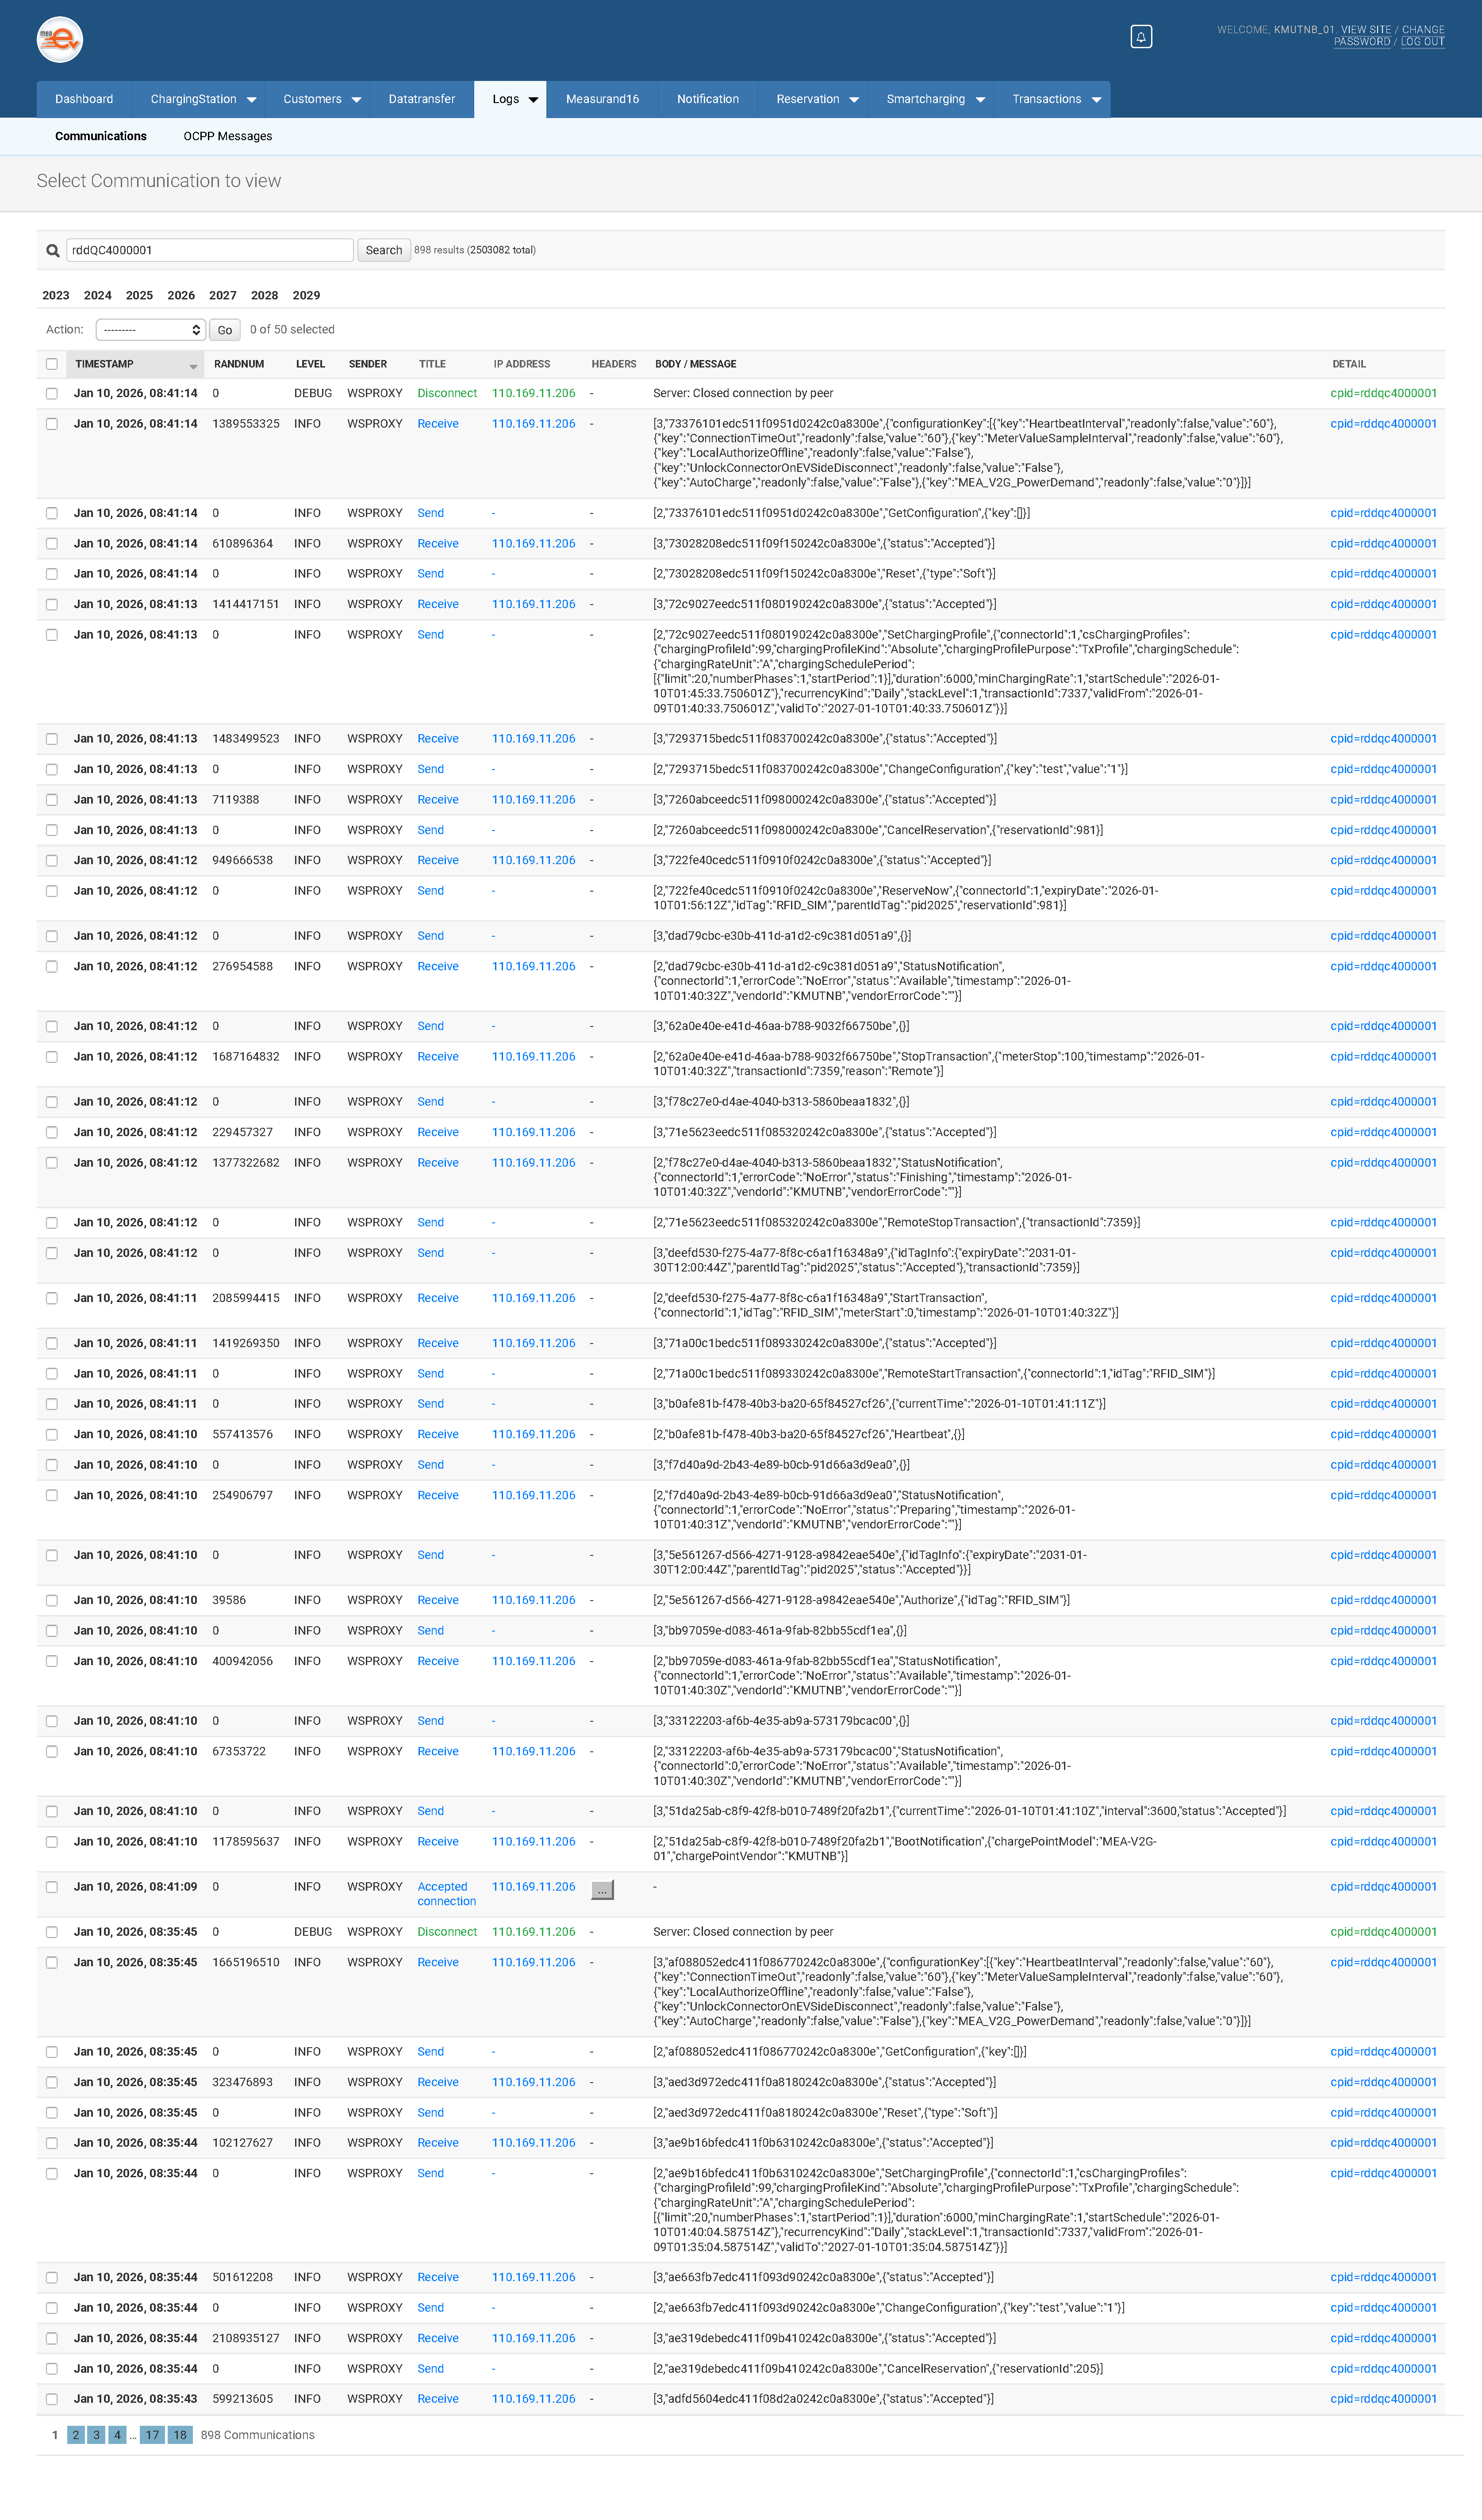
\includepdf[pages=1, viewport=0 459.4773109243697 1608.0 2735.0, clip, scale=0.85, pagecommand={\thispagestyle{plain}}, frame=true, linkname=server_log_comms.pdf_0]{server_log_comms.pdf}
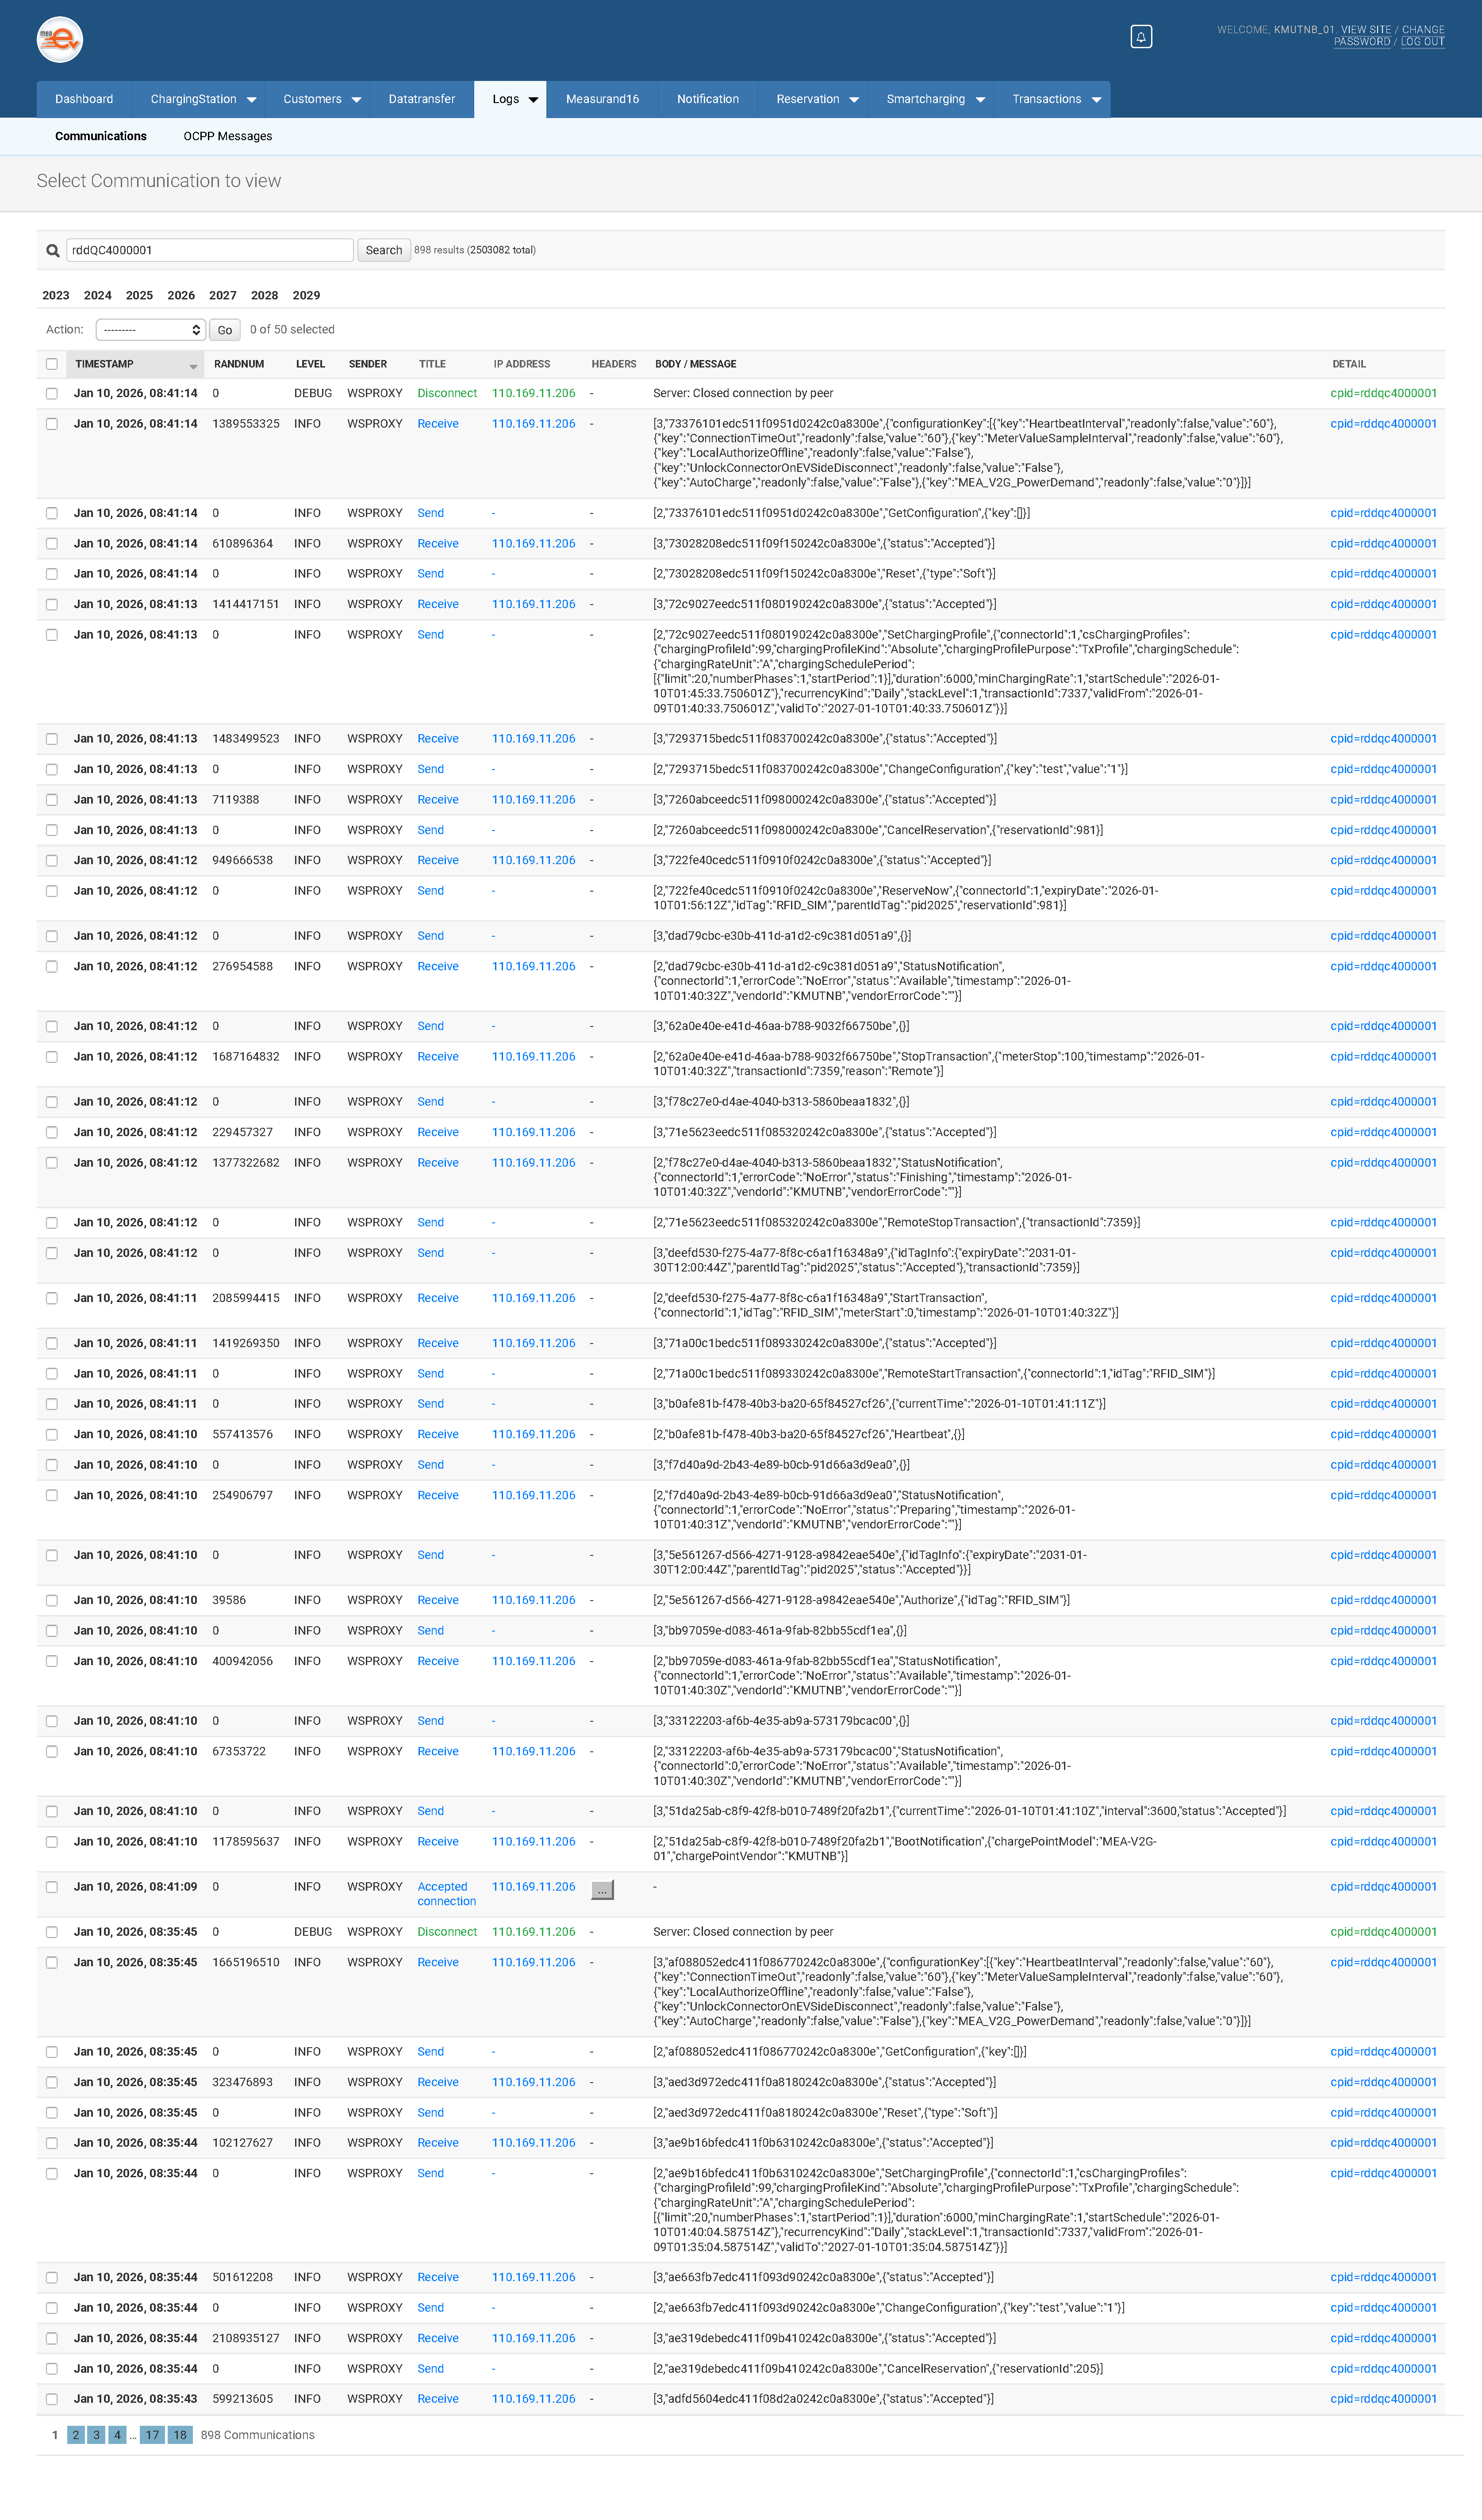
\includepdf[pages=1, viewport=0 0 1608.0 459.4773109243697, clip, scale=0.85, pagecommand={\thispagestyle{plain}}, frame=true, linkname=server_log_comms.pdf_1]{server_log_comms.pdf}

\end{document}
